\documentclass{aiaa-tc}% insert '[draft]' option to show overfull boxes

\usepackage{graphicx}
\usepackage{amsmath}
\usepackage{calc}%allows for scaling figures with integer division/multiplication of existing lengths

\title{Design and Manufacture of an Open-Hardware 
 	University Rocket Airframe using Carbon Fiber}

\author{
Joseph Shields, Brandon Bonner, Leslie Elwood, Erik Nelson, and Jacob East
	\thanks{Portland State University, Portland, OR 97201}
 }
% Data used by 'handcarry' option if invoked
\AIAApapernumber{2016}
\AIAAconference{Conference Name, Date, and Location}
\AIAAcopyright{\AIAAcopyrightD{2016}}
 
% Define commands to assure consistent treatment throughout document
\newcommand{\eqnref}[1]{(\ref{#1})}
\newcommand{\class}[1]{\texttt{#1}}
\newcommand{\package}[1]{\texttt{#1}}
\newcommand{\file}[1]{\texttt{#1}}
\newcommand{\BibTeX}{\textsc{Bib}\TeX}
\newcommand{\cots}{commercial off-the-shelf}
\newcommand{\weightReduction}{80\%}
\newcommand{\strengthIncrease}{??\%}

\begin{document}
\maketitle

\begin{abstract}
The amateur and university rocketry communities are rapidly reaching higher altitudes with more sophisticated rockets. However, most groups are still using heavy airframes made of metal or fiberglass. Commercial off-the-shelf airframes are either too expensive for low-budget university groups or too small to use as a platform for high altitude experiments. 
A capstone team of mechanical engineering seniors at Portland State University is developing a low-weight, modular carbon fiber airframe as an open-hardware technology for university rocketry. This team is continuing the work of a 2014 capstone team, who developed a carbon fiber layup process with promising results. 
This will enable low-budget groups like the Portland State Aerospace Society to explore high altitude science and compete in the university space race.  \end{abstract}
%\section*{Nomenclature}

\begin{figure}
\centering
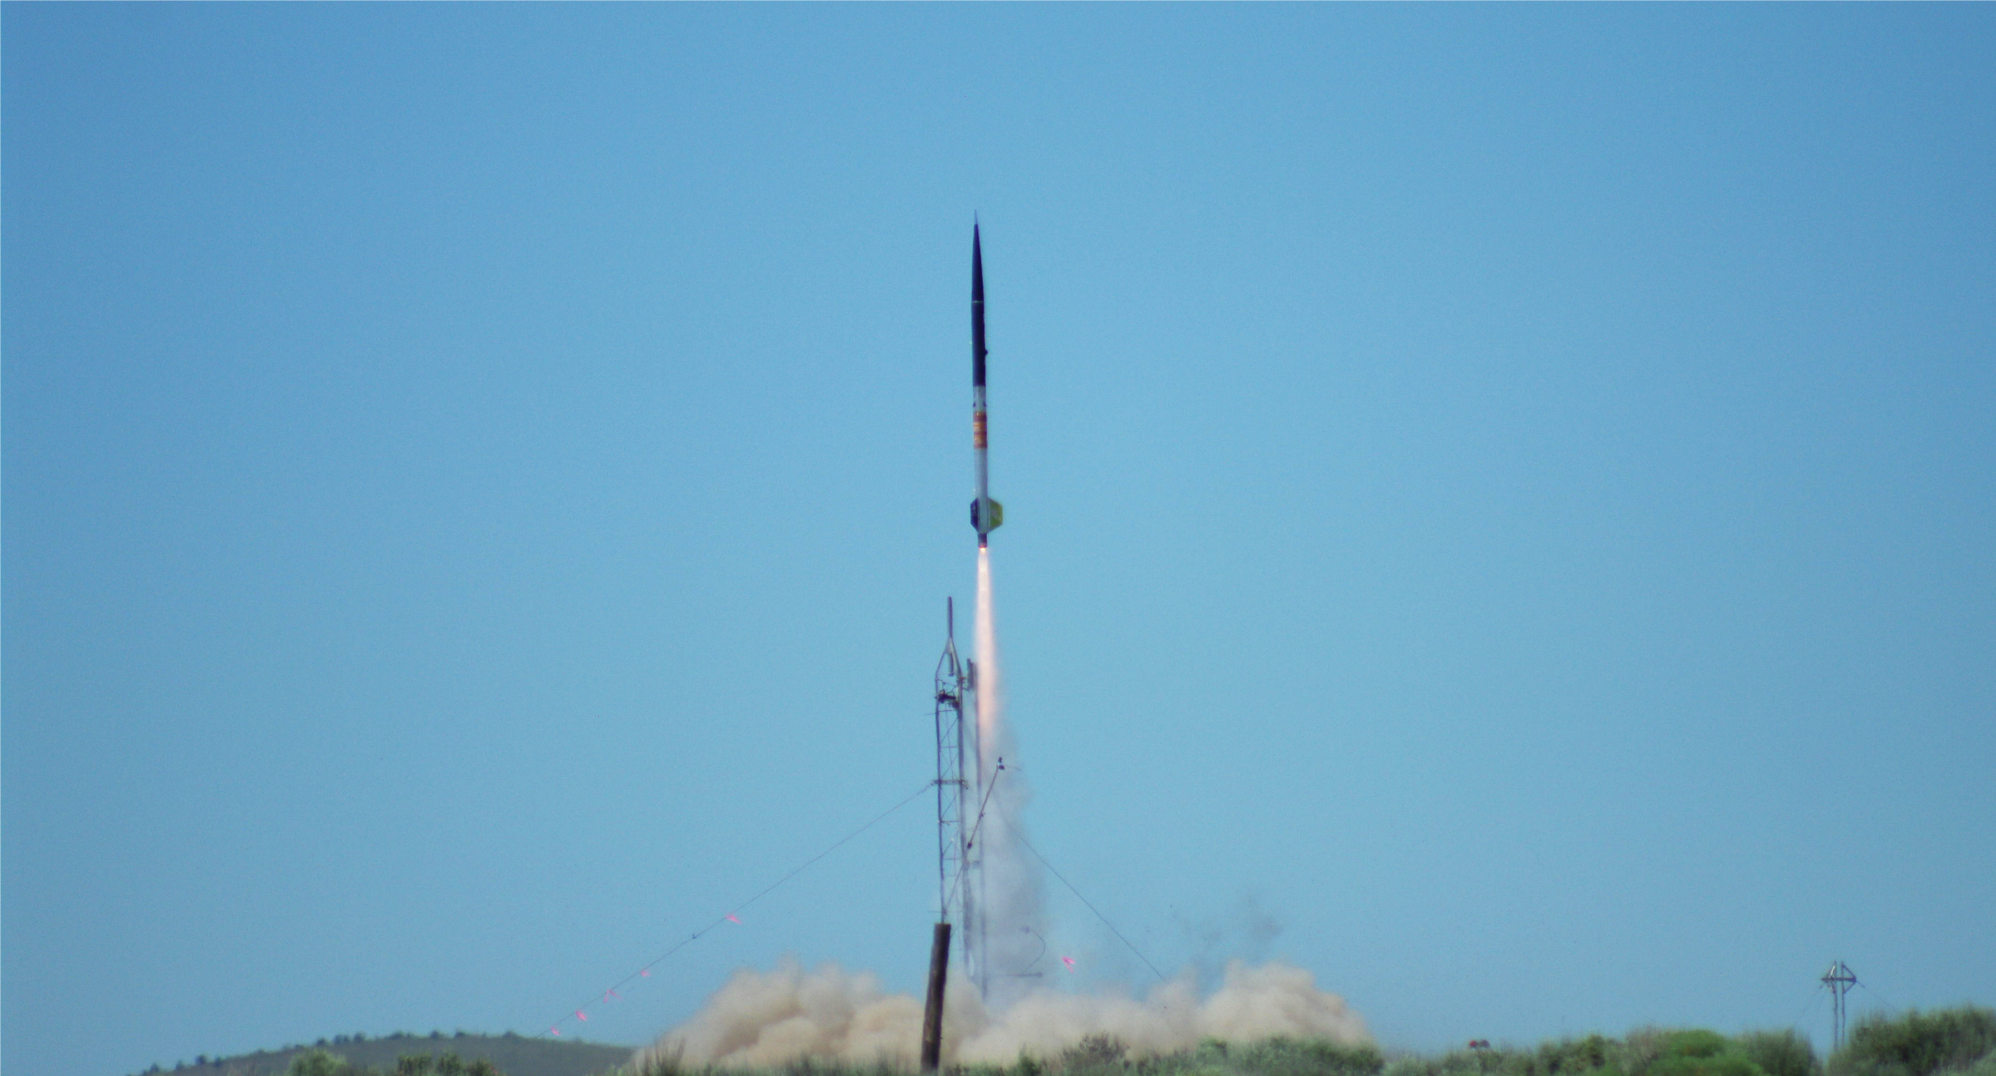
\includegraphics[width=\linewidth]{img/Jun2013_launch.jpg}
\caption{PSAS's LV2 rocket lifting off for the group's $11^\text{th}$launch.}
\label{fig:L-12}
\end{figure}

\section{Introduction}
The Portland State Aerospace Society is an interdisciplinary group of engineering students and alumni of Portland State University with the long term goal of putting a cubesat into orbit with their own rocket. 
% info about cubesat market growth: http://www.spaceref.com/news/viewpr.html?pid=44940 
Their current airframe, named LV2, has served for over 12 years, representing 10 of the group's 13 launches, and hosted experiments ranging from custom patch antennas and long range WiFi technology to GPS navigation and a cold gas reaction controll system. The LV2 platform is mostly constructed of aluminum with a fiberglass shell, with many of the parts having been fabricated in home garages. This makes for a robust but heavy design. Additionally, this airframe is built with a 4.5 inch inner diameter which PSAS's experiments have outgrown. 

The new airframe being designed, named LV3, aims to address these issues. The LV3 platform uses a 6 inch inner diameter, modules composed of carbon fiber and thin aluminum coupling rings, a carbon fiber nose cone, and a carbon fiber fin section. All of the airframe components connect via standardized rings, to accomodate future experimental modules and flight configurations.

The cylindrical LV3 airframe modules already outperform the old design with an \weightReduction{} reduction in weight and \strengthIncrease{} increase in yield strength. 
% Do we know what the increase in strength is? Also, can we confirm the weight reduction?
\section{Significance}

\section{Plan of Work}

\end{document}
